\documentclass[conference]{IEEEtran}
\IEEEoverridecommandlockouts
% The preceding line is only needed to identify funding in the first footnote. If that is unneeded, please comment it out.
\usepackage{cite}
\usepackage{amsmath,amssymb,amsfonts}
\usepackage{algorithmic}
\usepackage{textcomp}
\usepackage{theorem,caption,extarrows,mathrsfs,physics,bm}
\usepackage{graphicx,xcolor,booktabs,subfigure,tikz}
\usepackage{pgfplots,grffile}
\usepackage{fontspec}
\setmainfont{TeX Gyre Termes}
\usepackage[skins]{tcolorbox}
\usepackage{listings}
\lstset{
    basicstyle          =   \sffamily,          % 基本代码风格
    keywordstyle        =   \bfseries,          % 关键字风格
    commentstyle        =   \rmfamily\itshape,  % 注释的风格,斜体
    stringstyle         =   \ttfamily,  % 字符串风格
    flexiblecolumns,                % 别问为什么,加上这个
    numbers             =   left,   % 行号的位置在左边
    showspaces          =   false,  % 是否显示空格,显示了有点乱,所以不现实了
    numberstyle         =   \tiny\ttfamily,    % 行号的样式,小五号,tt等宽字体
    showstringspaces    =   false,
    captionpos          =   t,      % 这段代码的名字所呈现的位置,t指的是top上面
    frame               =   shadowbox,   % 显示边框
    rulesepcolor=\color{red!20!green!20!blue!20}
}

\lstdefinestyle{Python}{
    language        =   Python, % 语言选Python
    backgroundcolor=\color{backpycol},
    basicstyle      =   \ttfamily,
    numberstyle     =   \ttfamily,
    keywordstyle    =   \color{blue},
    keywordstyle    =   [2] \color{teal},
    stringstyle     =   \color{magenta},
    commentstyle    =   \color[HTML]{338AAF}\ttfamily,
    breaklines      =   true,   % 自动换行,建议不要写太长的行
    columns         =   fixed,  % 如果不加这一句,字间距就不固定,很丑,必须加
    basewidth       =   0.5em,
}
\definecolor{codegreen}{rgb}{0,0.6,0}
\definecolor{codegray}{rgb}{0.5,0.5,0.5}
\definecolor{codepurple}{rgb}{0.58,0,0.82}
\definecolor{backcolour}{rgb}{0.95,0.95,0.92}
\definecolor{backpycol}{rgb}{0.97,0.95,0.97}
\lstdefinestyle{C++}{
    language =[ANSI]C,
    backgroundcolor=\color{backcolour},
    commentstyle=\color[HTML]{338AAF}\ttfamily,
    keywordstyle=\sffamily\bfseries\color{magenta},
    numberstyle=\color{codegray},
    stringstyle=\color{codepurple},
    basicstyle=\ttfamily,
    breakatwhitespace=false,
    breaklines=true,
    basewidth=0.5em,
    captionpos=b,
    columns=fixed,
    frame=shadowbox,
    keepspaces=true,
    numbers=left,
    numbersep=5pt,
    showspaces=false,
    showstringspaces=false,
    showtabs=false,
    tabsize=4
}
\lstdefinestyle{matlab}{
    language=matlab,
    backgroundcolor=\color{backcolour},
    commentstyle=\color[HTML]{338AAF}\ttfamily,
    keywordstyle=\sffamily\bfseries\color{magenta},
    numberstyle=\color{codegray},
    stringstyle=\color{codepurple},
    basicstyle=\ttfamily,
    breakatwhitespace=false,
    breaklines=true,
    basewidth=0.5em,
    captionpos=b,
    columns=fixed,
    keepspaces=true,
    numbers=left,
    numbersep=5pt,
    showspaces=false,
    showstringspaces=false,
    showtabs=false,
    tabsize=4,
    frame=shadowbox
}
\definecolor{mygreen}{rgb}{0,0.6,0}
\definecolor{mygray}{rgb}{0.5,0.5,0.5}
\definecolor{mymauve}{rgb}{0.58,0,0.82}
\definecolor{bggray}{rgb}{0.93,0.95,0.94}
\lstdefinestyle{pseudocode}{
    backgroundcolor=\color{bggray},
    columns=fullflexible,
    tabsize=4,
    breaklines=true,               % automatic line breaking only at whitespace
    captionpos=b,                  % sets the caption-position to bottom
    commentstyle=\color{mygreen},  % comment style
    escapeinside={\%*}{*)},        % if you want to add LaTeX within your code
    keywordstyle=\color{blue},     % keyword style
    stringstyle=\color{mymauve}\ttfamily,  % string literal style
    frame=shadowbox,
    rulesepcolor=\color{red!20!green!20!blue!20},
    % identifierstyle=\color{red},
    language=c++,
    numbers=left,
    numberstyle=\small\color{codegray},
    basicstyle=\ttfamily,% size of fonts used for the code
    escapeinside=``,
    xleftmargin=0.6em,
    xrightmargin=0.6em,
    aboveskip=1em
}
\lstdefinestyle{Fortran}{
    language =fortran,
    backgroundcolor=\color{backcolour},
    commentstyle=\color[HTML]{338AAF}\ttfamily,
    keywordstyle=\sffamily\bfseries\color{magenta},
    numberstyle=\small\color{codegray},
    stringstyle=\color{codepurple},
    basicstyle=\ttfamily,
    breakatwhitespace=false,
    breaklines=true,
    basewidth=0.5em,
    captionpos=b,
    columns=fixed,
    frame=shadowbox,
    keepspaces=true,
    numbers=left,
    numbersep=5pt,
    showspaces=false,
    showstringspaces=false,
    showtabs=false,
    tabsize=4
}
\setmonofont{CMU Typewriter Text}
\pgfplotsset{compat=newest}
  %% the following commands are needed for some matlab2tikz features
\usetikzlibrary{plotmarks}
\usetikzlibrary{arrows.meta}
\usetikzlibrary{calc}
\usepgfplotslibrary{patchplots}
\def\BibTeX{{\rm B\kern-.05em{\sc i\kern-.025em b}\kern-.08em
    T\kern-.1667em\lower.7ex\hbox{E}\kern-.125emX}}
%% Define the theorem and proof
\newtheorem{theorem}[subsection]{Theorem}
\newtheorem{definition}[subsection]{Definition}
\newenvironment{thmbox}{\par
	\vspace{4pt}
	\begin{center}
	\tcbset{enhanced,notitle,colframe=black,colback=white}
	\begin{tcolorbox}[fuzzy shadow={1.6mm}{-1.6mm}{0mm}{0mm}{fill=black!90!white},arc=0mm]}{\end{tcolorbox}
	\end{center}}
\begin{document}

\title{Digital Signal Processing Lab Report 2}

\author{\IEEEauthorblockN{1\textsuperscript{st} Qiu Kunyuan}
	\IEEEauthorblockA{\textit{Department of EEE. } \\
		\textit{Southern University of Science and Technology}\\
		Shenzhen, PRC \\
		11913019@mail.sustech.edu.cn}
}

\maketitle

\begin{abstract}
	This lab aims to the demonstration of DT(Discrete-Time) systems under the MATLAB\(\circledR \) programming environment and exploration of essential characteristics of DT systems using MATLAB. In this lab session, the DT system modeling and analysis method is applied to discretizing
	CT(Continuous Time) functions, solving basic difference equations, filter building and modeling the stock market. Additionally, a black-box system goes under test and being analyzed in this lab with DT system testing and analysis methods.
\end{abstract}

\begin{IEEEkeywords}
	discrete-time system, MATLAB, system modeling, difference equation, black-box system
\end{IEEEkeywords}

\section{Introduction}

\subsection{Discrete-Time System}

A DT system is any mapping \(S:x\mapsto y\)that maps a discrete-time input \(x[t]\) to a discrete-time output \(y[t]\). Digital computers can and can only store or process DT systems, due to all the quantities and signals expressed in these computers must be digitized and discretized.

Analog systems may process \textit{raw}, referring continuous-time, CT signals directly with infinite sampling frequency, but analog systems are unable to be reconfigured quickly comparing to digital systems, while the parameters of analog systems drifts along with the time and results in the degenerate of accuracy.

Mathematically, the DT systems are mostly expressed in difference equations
\begin{equation}
	y[t]=\mathcal{S} (x[t],y[t])
\end{equation}
and the notation \(\mathcal{S}(x) \) is often used to denote DT systems. Block diagrams are also used to express DT systems, making it possible to obtain an intuitive view of system structure while reserving the mathematical characteristics of the system.

\subsection{Analyzing DT System}
A DT system might be linear or nonlinear, time variant or time invariant, causal or noncausal, memoryless or with-memory, active or passive, and stable or unstable. These properties can be written in formulas strictly and verified mathematically by deduction.

\begin{theorem}[Property of Linear System]
	\label{linear_prop}
	\begin{thmbox}
		A system is linear, iff the system satisfies both additivity and homogeneity:
		\begin{equation}
			\mathcal{S} \left( \sum_{i}^{}\alpha_{i}x_{i} \right) =\alpha_{i}\sum_{i}^{}S(x_{i})
		\end{equation}
	\end{thmbox}
\end{theorem}

\begin{theorem}[Property of Time-Invariant System]
	\label{ti_prop}
	\begin{thmbox}
		A system is time-invariant, if the output of the system only delays for the same time to the delay of the input:
		\begin{equation}
			y(t)= \mathcal{S} (x(t))\Rightarrow y(t-t_{0})= \mathcal{S} (x(t-t_{0}))
		\end{equation}
	\end{thmbox}
\end{theorem}

A system is called as Linear Time-Invariant(LTI) if the system both satisfies linearity and time-invariance. For LTI system, the output of the DT system is uniquely determined by the impulse response of the system, and can be evaluated closely in forms of \textit{convolution}:
\begin{equation}
	y[t]=x[t] * \mathcal{S}[\delta[t]]
\end{equation}

However, numerical solution of DT system with computer does not require LTI property since solving difference equations in computer are simple cumulative summation, that can be easily realized by loop. In MATLAB realizations of difference equation solver, the built-in \lstinline{cumsum} function are frequently used since it adopted BLAS libraries to accelerate the vector operations dramatically.

\section{Background Exercises}

\subsection{Example DT Systems}

Use DT systems to approximate the CT differentiator and integrator.

\paragraph{Problem (i)(ii)}

For CT differentiator, this system can be approximated by a 1st-order FIR. In difference equation form, the FIR is
\begin{equation}
	y[t]=x[t]-x[t-1]
\end{equation}\pagebreak

Use MATLAB to demonstrate the approximation by plotting the result of the differentiator:
\begin{figure}[htpb]
	\begin{center}
		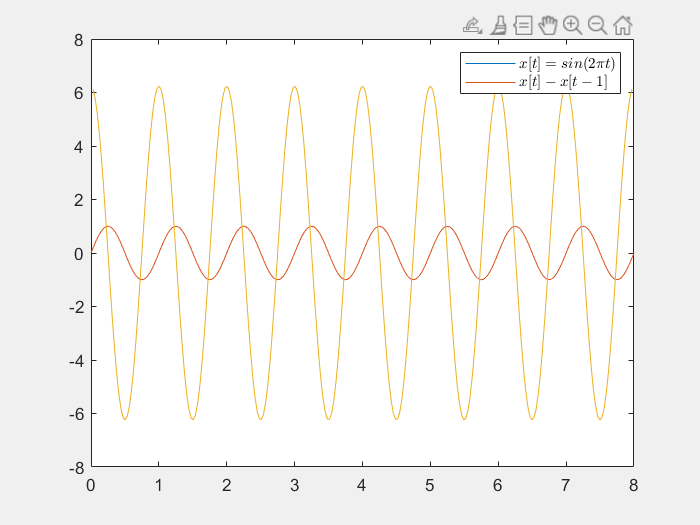
\includegraphics[width=0.45\textwidth]{../matlab/q221_1.png}
		\caption{MATLAB plot of a DT differentiator}
		\label{fig:1}
	\end{center}
\end{figure}

For CT integrator, this system can be approximated by a 1st-order IIR. To write the integrator(or accumulator) in closed form, the filter is expressed in IIR form
\begin{equation}
	y[t]=y[t-1]=x[t]
\end{equation}

Use MATLAB to demonstrate the approximation by plotting the result of the integrator:
\begin{figure}[htpb]
	\begin{center}
		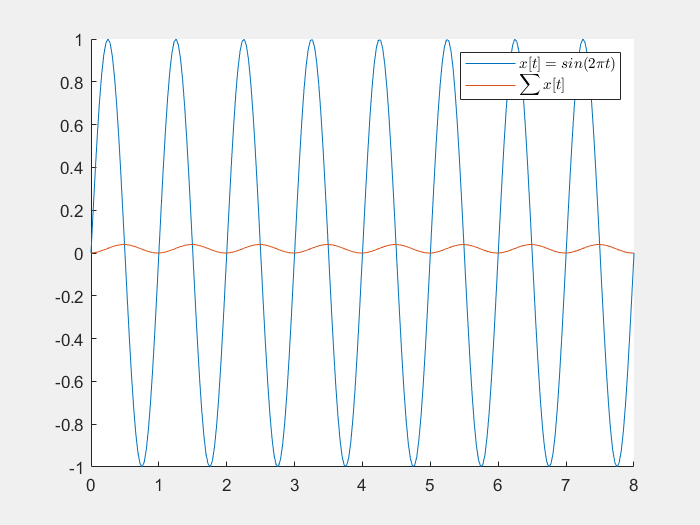
\includegraphics[width=0.45\textwidth]{../matlab/q221_2.png}
		\caption{MATLAB plot of a DT integrator}
		\label{fig:2}
	\end{center}
\end{figure}

\paragraph{Problem (iii)}

Diagram of differentiator:
\begin{figure}[htpb]
	\begin{center}
		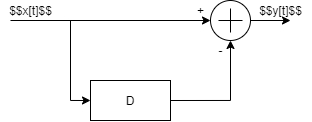
\includegraphics[width=0.32\textwidth]{221-dif.png}
		\caption{Block diagram of differentiator}
		\label{fig:3}
	\end{center}
\end{figure}

Diagram of integrator:
\begin{figure}[htpb]
	\begin{center}
		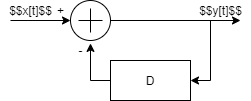
\includegraphics[width=0.36\textwidth]{221-int.png}
		\caption{Block diagram of integrator}
		\label{fig:4}
	\end{center}
\end{figure}
\subsection{Stock Market Example}
\paragraph{Method 2.3}
Difference equation:
\begin{equation}
	y[t]=\frac{1}{3}(x[t]+x[t-1]+x[t-2])
\end{equation}

The diagram of this system is
\begin{figure}[htpb]
	\begin{center}
		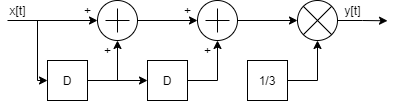
\includegraphics[width=0.4\textwidth]{222-1.png}
		\caption{Block diagram of system (2.3)}
		\label{fig:5}
	\end{center}
\end{figure}

Use MATLAB to evaluate the impulse response:
\begin{lstlisting}[language=matlab,style=matlab]
	b1 = [1, 1, 1] * 1/3;
	a1 = 1;
	t = 0:10;
	d1 = impseq(t(1), 0, t(end));
	y1 = filter(b1, a1, d1);
	fig = figure(1);
	stem(t, y1);
	legend('Method 2.3');
\end{lstlisting}
\begin{figure}[htpb]
	\begin{center}
		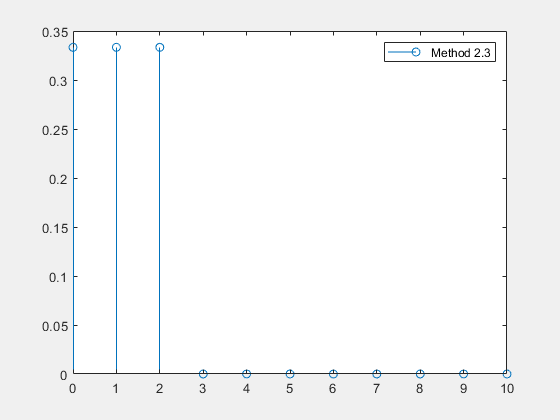
\includegraphics[width=0.45\textwidth]{../matlab/q222_1.png}
		\caption{Impulse response of method 2.3}
		\label{fig:6}
	\end{center}
\end{figure}
\pagebreak
\paragraph{Method 2.4}
Difference equation of the system:
\begin{equation}
	y[t]-0.8y[t-1]=0.2x[t]
\end{equation}

The diagram of the system is
\begin{figure}[htpb]
	\begin{center}
		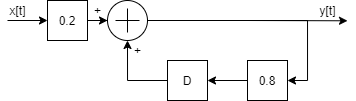
\includegraphics[width=0.4\textwidth]{222-2.png}
		\caption{Block diagram of system (2.4)}
		\label{fig:7}
	\end{center}
\end{figure}

Use MATLAB to evaluate the impulse response. The evaluating code is identical to the code used in Problem 2.3, while the only difference is the different coefficients:
\begin{lstlisting}[language=matlab,style=matlab]
	b2 = 1 * 0.2;
	a2 = [1, -0.8];
	t = 0:15;
\end{lstlisting}

Plotting result:
\begin{figure}[htpb]
	\begin{center}
		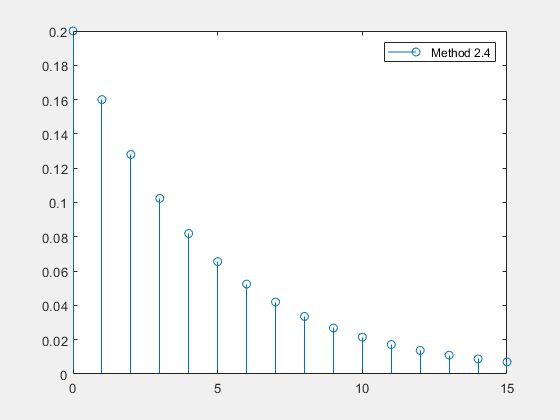
\includegraphics[width=0.45\textwidth]{../matlab/q222_2.png}
		\caption{Impulse response of method 2.4}
		\label{fig:8}
	\end{center}
\end{figure}

\paragraph{Method 2.5}
Difference equation of the system:
\begin{equation}
	y[t]-y[t-1]=\frac{1}{3}x[t]-\frac{1}{3}x[t-3]
\end{equation}
\begin{figure}[htpb]
	\begin{center}
		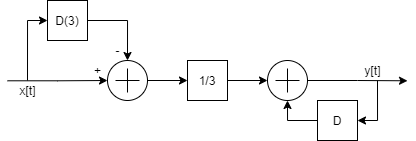
\includegraphics[width=0.4\textwidth]{222-3.png}
		\caption{Block diagram of system (2.5)}
		\label{fig:9}
	\end{center}
\end{figure}

Use MATLAB to evaluate the impulse response.
\begin{lstlisting}[language=matlab,style=matlab]
	b3 = [1, 0, 0, -1] * 1/3;
	a3 = [1, -1];
	t = 0:10;
\end{lstlisting}
\begin{figure}[htpb]
	\begin{center}
		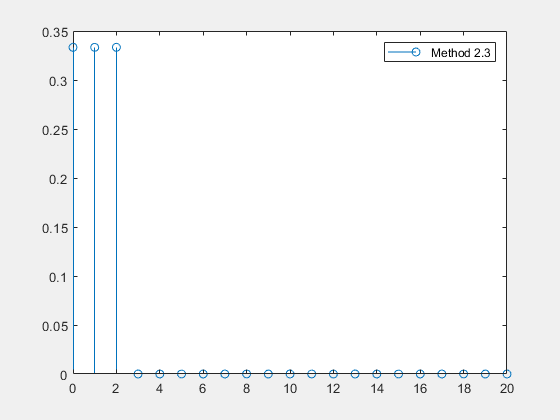
\includegraphics[width=0.45\textwidth]{../matlab/q222_3.png}
		\caption{Impulse response of method 2.4}
		\label{fig:10}
	\end{center}
\end{figure}

\paragraph{Moving Averages}
For the methods (2.3), the output \(y[t]\) is the mean value of the nearest inputs, and the window length of the input is 3. Therefore, this method is \textit{moving average}.

For the method (2.5), use Z-transform to simplify the IIR filter:
\begin{equation}
	\begin{aligned}
		Y[z] & =z^{-1}Y[z]+\frac{x[z]}{3}-z^{-3}\frac{x[z]}{3} \\
		     & =\frac{1-z^{-3}}{3(1-z^{-1})}X[z]               \\
		     & =\frac{1}{3}(1+z^{-1}+z^{-2})X[z]
	\end{aligned}
\end{equation}
Therefore in time domain, the system is
\begin{equation}
	y[t]=\frac{1}{3}(x[t]+x[t-1]+x[t-2])
\end{equation}
, which is a moving average.

\section{Example DT systems}

MATLAB code for signal processing:
\begin{lstlisting}[language=matlab, style=matlab]
	x1=signal;
	dx1 = [x1(1), diff(x1)];
	%differentiator
	ix1 = cumsum(x1);
	%integrator
\end{lstlisting}

(a) For system (1)

\begin{equation}
	x_{1}[t]=\delta [t]-\delta [t-5]
\end{equation}

The differentiation result are two impulse pairs and the integration result is a box function.
\begin{figure}[htpb]
	\begin{center}
		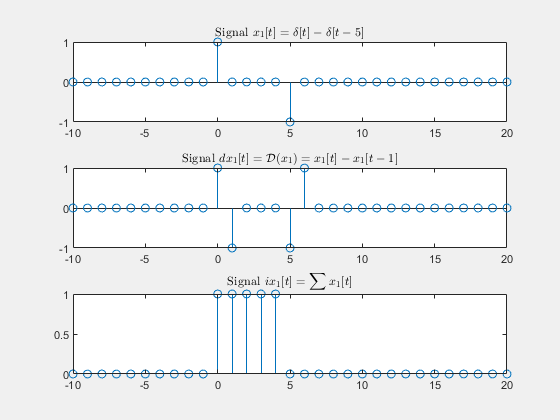
\includegraphics[width=0.45\textwidth]{../matlab/q23_1.png}
		\caption{Difference and integration result of signal \(x_{1}[t]\)}
		\label{fig:11}
	\end{center}
\end{figure}

(b) For system (2)
\begin{equation}
	x_{2}[t]=u[t]-u[t-(N+1)],\ N=10
\end{equation}
the differentiation result are 2 impulses and the integration result is a ramp function connected by a Heaviside step function.
\begin{figure}[htpb]
	\begin{center}
		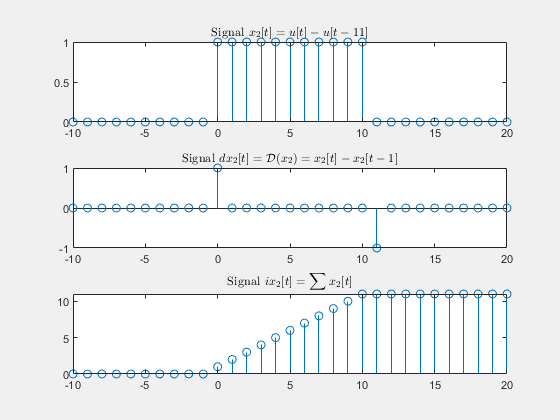
\includegraphics[width=0.45\textwidth]{../matlab/q23_2.png}
		\caption{Difference and integration result of signal \(x_{2}[t]\)}
		\label{fig:12}
	\end{center}
\end{figure}

\section{Difference Equations}
\paragraph{Case 1}
The system \(\mathcal{S}_{1}\) is a differentiator. Therefore, its system diagram is
\begin{figure}[htpb]
	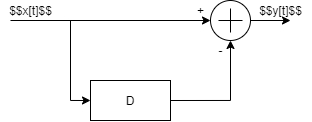
\includegraphics[width=0.35\textwidth]{221-dif.png}
	\caption{System diagram of \(\mathcal{S}_{1}\)}
	\label{fig:13}
\end{figure}

The impulse response of the system is an impulse pair, plotted by MATLAB and shown below:
\begin{figure}[htpb]
	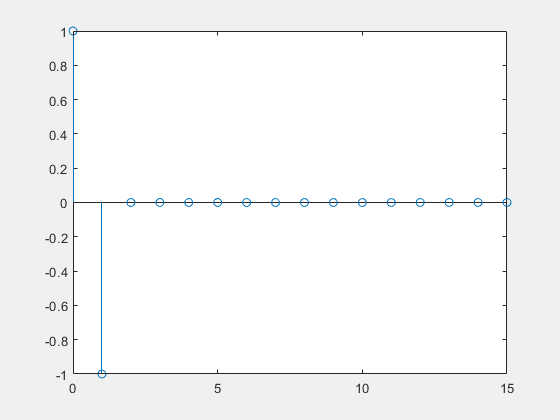
\includegraphics[width=0.45\textwidth]{../matlab/q24_1.png}
	\caption{Impulse response of system \(\mathcal{S}_{1}\)}
	\label{fig:14}
\end{figure}

\paragraph{Case 2}
The system \(\mathcal{S}_{2}\) is a 1st-order IIR filter. Its system diagram is
\begin{figure}[htpb]
	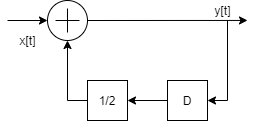
\includegraphics[width=0.45\textwidth]{24-2.png}
	\caption{System diagram of \(\mathcal{S}_{2}\)}
	\label{fig:15}
\end{figure}

The impulse response of this filter is an attenuating power function. Use MATLAB to plot the response:
\begin{figure}[htpb]
	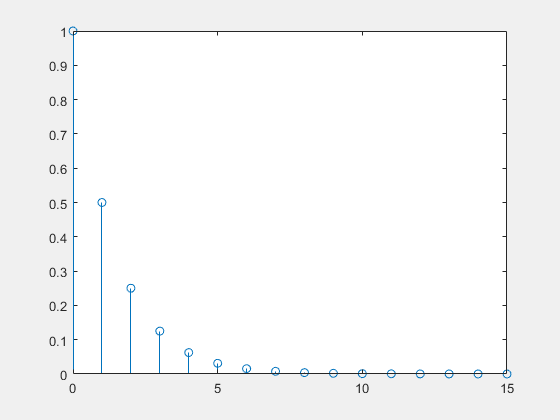
\includegraphics[width=0.45\textwidth]{../matlab/q24_2.png}
	\caption{Impulse response of system \(\mathcal{S}_{2}\)}
	\label{fig:16}
\end{figure}

\paragraph{Case 3}
The system \(\mathcal{S}_{3}\) is the serial connection of system \(\mathcal{S}_{1}\) and \(\mathcal{S}_{2}\). Therefore, this system is a general digital filter
containing one FIR loop and one IIR loop.
\begin{figure}[htpb]
	\begin{small}
		\begin{center}
			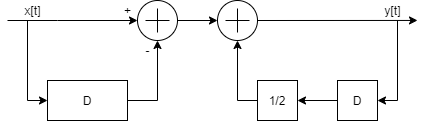
\includegraphics[width=0.35\textwidth]{24-3.png}
		\end{center}
		\caption{System diagram of system \(\mathcal{S}_{3}\)}
		\label{fig:17}
	\end{small}
\end{figure}


Use MATLAB to evaluate and plot the impulse of this system:
\begin{figure}[htpb]
	\begin{small}
		\begin{center}
			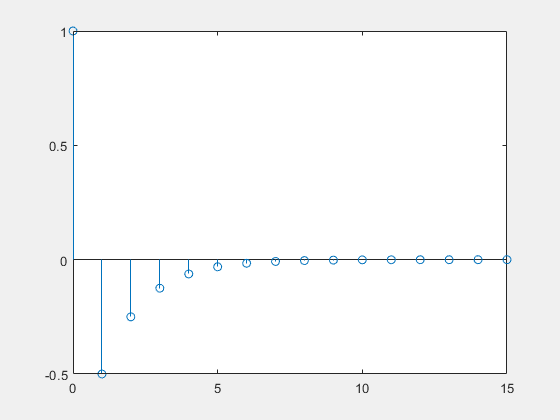
\includegraphics[width=0.45\textwidth]{../matlab/q24_3.png}
		\end{center}
		\caption{Impulse response of system \(\mathcal{S}_{3}\)}
		\label{fig:18}
	\end{small}
\end{figure}

\paragraph{Case 4}
The system \(\mathcal{S}_{4}\) is the serial connection of system \(\mathcal{S}_{2}\) and \(\mathcal{S}_{1}\). Its structure is nearly identical to system \(\mathcal{S}_{3}\):
\begin{figure}[htpb]
	\begin{small}
		\begin{center}
			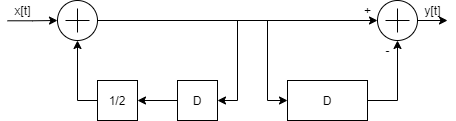
\includegraphics[width=0.35\textwidth]{24-4.png}
		\end{center}
		\caption{System diagram of system \(\mathcal{S}_{4}\)}
		\label{fig:19}
	\end{small}
\end{figure}

Use MATLAB to plot the impulse of this system:

\begin{figure}[htb]
	\begin{small}
		\begin{center}
			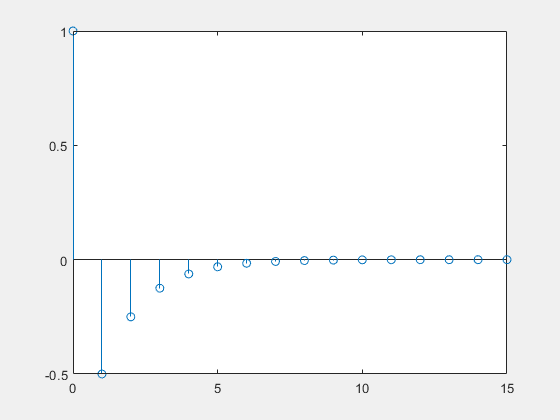
\includegraphics[width=0.25\textwidth]{../matlab/q24_4.png}
		\end{center}
		\caption{Impulse Response of system \(\mathcal{S}_{4}\)}
		\label{fig:20}
	\end{small}
\end{figure}
Compare this response with the response of the previous system, it's easy to find that the response of system \(\mathcal{S}_{2}(\mathcal{S}_{1})\) is identical as \(\mathcal{S}_{1}(\mathcal{S}_{2})\).
This is evident to the commutativity of two serial LTI systems.

\paragraph{Case 5}
The system \(\mathcal{S}_{5}\) is the addition of the filter coefficients of system \(\mathcal{S}_{2}\) and \(\mathcal{S}_{1}\). The structure of this new system is completely different to system \(\mathcal{S}_{1}\) or \(mathcal{S}_{2}\),
therefore its response is consequently different.

\begin{figure}[htpb]
	\centering
	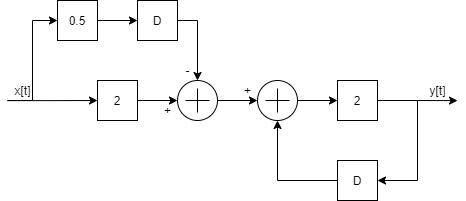
\includegraphics[width=0.45\textwidth]{24-5.png}
	\caption{System diagram of system \(\mathcal{S}_{5}\)}
	\label{fig:21}
\end{figure}

Use MATLAB to plot the impulse of this system:

\begin{figure}[htpb]
	\begin{small}
		\begin{center}
			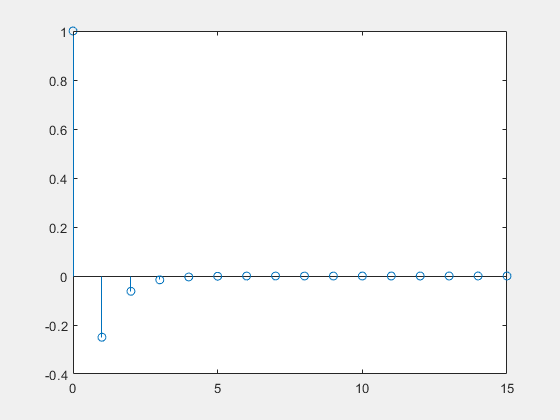
\includegraphics[width=0.45\textwidth]{../matlab/q24_5.png}
		\end{center}
		\caption{Impulse response of system \(\mathcal{S}_{5}\)}
		\label{fig:22}
	\end{small}
\end{figure}
This response is different to the response of paralleled system composed by \(\mathcal{S}_{1}\) and \(\mathcal{S}_{2}\), for the system analyzed above is addition of the filter coefficients of the two components.

\section{Audio Filtering}

Use the \lstinline{audioread()}(which replaces the \lstinline{auread()} in newer versions of MATLAB) command to load the audio file into MATLAB, and use \lstinline{sound()} command to play this audio.

From the coefficient of the filter, it's easy to infer that the system \( \mathcal{\MakeUppercase{S}}_{1} \) is a differentiator that blocks the low-frequency components of the input signal. The frequency response of \(\mathcal{S}_{1}\), as Fig.\ref{fig:resp_s1} shows, is a 1st-order low-pass filter. And the system \( \mathcal{S}_{2} \), with the frequency response shown in Fig.\ref{fig:resp_s2}, is a low-pass filter that blocks the high-frequency components of the input signal.

Therefore, we can anticipate the effect of the two filters. The output of the filter \(\mathcal{S}_{1}\) hears should be sharper than input due to the decreased low frequency components, while the output of filter \( \mathcal{S}_{2} \) should be more mellow than input.

The frequency response of the two filters are evident to the anticipations above:

\begin{figure}[htpb]
	\begin{small}
		\begin{center}
			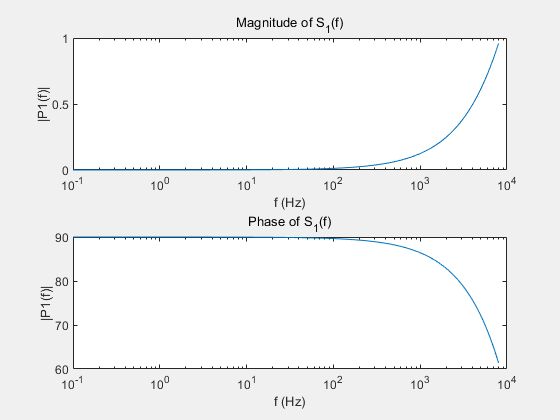
\includegraphics[width=0.45\textwidth]{../matlab/q25_3.png}
		\end{center}
		\caption{Frequency response of \(\mathcal{S}_{1}\)}
		\label{fig:resp_s1}
	\end{small}
\end{figure}

\begin{figure}[htpb]
	\begin{small}
		\begin{center}
			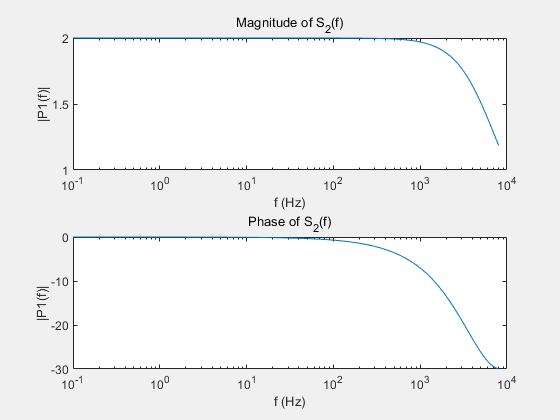
\includegraphics[width=0.45\textwidth]{../matlab/q25_4.png}
		\end{center}
		\caption{Frequency response of \(\mathcal{S}_{2}\)}
		\label{fig:resp_s2}
	\end{small}
\end{figure}

Use the MATLAB code shown below to evaluate the output of the two filters and plot the frequency spectrum of the output.
\begin{lstlisting}[language=matlab,style=matlab]
	clear;close;clc;

	[y, Fs] = audioread("music.au");
	el = floor(length(y) / 2) * 2;
	f0 = Fs * (0:(el / 2)) / el;

	fy = fftSingle(y);
	fy(1) = 0;

	s1 = [[1, -1]; [1, 0]];
	s2 = [[1, 0]; [1, -0.5]];
	y1 = filter(s1(1, :), s1(2, :), y);
	y2 = filter(s2(1, :), s2(2, :), y);
	fy1 = fftSingle(y1);
	fy1(1) = 0;
	fy2 = fftSingle(y2);
	fy2(1) = 0;

	%Plotting the fft output;

	%Bode Plot
	w = logspace(-1, log10(Fs), 200);
	sys1 = tf(s1(1, :), s1(2, :), 1 / Fs);
	[mag, phase, wout] = bode(sys1, w);
	mag1 = mag(1, :);
	phase1 = phase(1, :);
	%Plot the Bode plot of System S1;

	sys2 = tf(s2(1, :), s2(2, :), 1 / Fs);
	[mag, phase, wout] = bode(sys2, w);
	mag2 = mag(1, :);
	phase2 = phase(1, :);
	%Plot the Bode plot of System S2;

	function fout = fftSingle(y)
    	el = floor(length(y) / 2) * 2;
    	fy = abs(fft(y) / length(y));
    	fy = fy(1:el);
    	fy = fy(1:(el / 2 + 1));
    	fy(2:(end - 1)) = 2 * fy(2:(end - 1));
    	fout = fy;
	end
\end{lstlisting}

To compare the output and input of each filter, the output and input are stacked in the same plot, and there are difference plots showing the subtraction of output and input.

The output of filter \(\mathcal{S}_{1}\) shown in Fig.\ref{fig:out_s1} meets the anticipation from the coefficients of \(\mathcal{S}_{1}\):

\begin{figure}[htpb]
	\begin{small}
		\begin{center}
			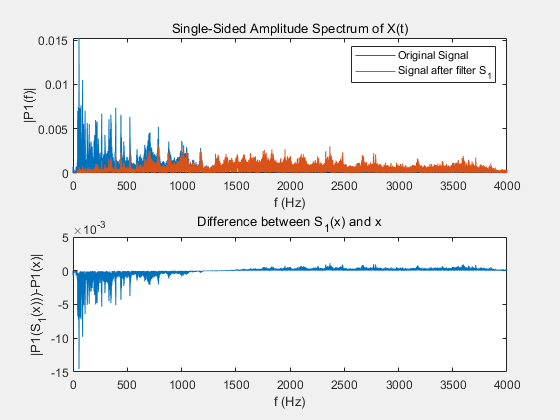
\includegraphics[width=0.45\textwidth]{../matlab/q25_1.png}
		\end{center}
		\caption{Output spectrum of \(\mathcal{S}_{1}(x(t))\)}
		\label{fig:out_s1}
	\end{small}
\end{figure}

And the output of filter \( \mathcal{S}_{2} \) shown in Fig.\ref{fig:out_s2} confirms the anticipation using the coefficients of \( S_{2} \):

\begin{figure}[htpb]
	\begin{small}
		\begin{center}
			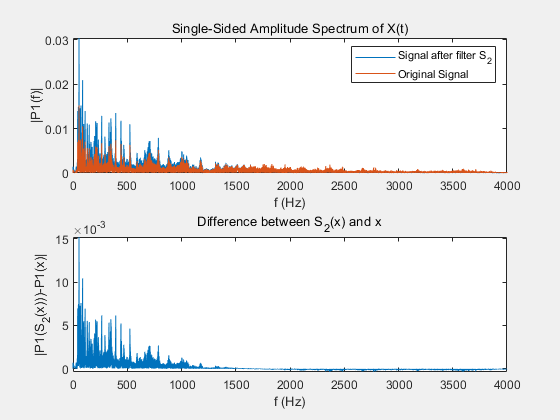
\includegraphics[width=0.45\textwidth]{../matlab/q25_2.png}
		\end{center}
		\caption{Output spectrum of \( \mathcal{S}_{2}(x(t)) \)}
		\label{fig:out_s2}
	\end{small}
\end{figure}

\section{Inverse System}
The definition of \textit{inverse system} is
\begin{theorem}[Inverse System]
	\label{thm:inv_sys}
	\begin{thmbox}
		A system \(\mathcal{A} \) is called the inverse system of the given system \(\mathcal{S} \), if and only if
		\begin{equation}
			\mathcal{A}(\mathcal{S}(x(t)))=x(t)
		\end{equation}
	\end{thmbox}
\end{theorem}
Use the z-Transformation of the impulse signal to acquire the inverse system \(\mathcal{S}^{-1}(t)\) of the given system \(\mathcal{S}(t)\):
\begin{equation}
	\begin{aligned}
		\mathcal{A}(\mathcal{S}(x(t)))                     & =x(t) \\
		\Leftrightarrow x(t)*\mathcal{A}(t)*\mathcal{S}(t) & =x(t) \\
		\Leftrightarrow \mathcal{A}(z)\mathcal{S}(z)       & =1    \\
	\end{aligned}
\end{equation}
Therefore, the inverse system in Z-domain can be easily obtained:
\begin{theorem}[Obtain the Inverse System]
	\begin{thmbox}
		The inverse system \(\mathcal{S}^{-1}(z)\) of a given transfer function \(\mathcal{S}(z)\) in Z-domain is:
		\begin{equation}
			\mathcal{S}^{-1}(z)=\frac{1}{\mathcal{S}(z)}
		\end{equation}
	\end{thmbox}
\end{theorem}

For the system
\begin{equation}
	\mathcal{S}_{2}(t):\ y[t]=\frac{y[t-1]}{2}+x[t]
\end{equation}
, its inverse system in Z-domain is
\begin{equation}
	\begin{aligned}
		\mathcal{S}_{2}^{-1}(z) & =\frac{1}{\mathcal{S}_{2}(z)}        \\
		                        & =\left( \frac{z}{z-0.5} \right)^{-1} \\
		                        & =1-\frac{1}{2z}
	\end{aligned}
\end{equation}
, and thus the inverse system in time domain is
\begin{equation}
	\mathcal{S}_{2}^{-1}(t):\ y[t]=x[t]-\frac{x[t-1]}{2}
\end{equation}

Use MATLAB to verify the correctness of this inversion:
\begin{figure}[htpb]
	\begin{small}
		\begin{center}
			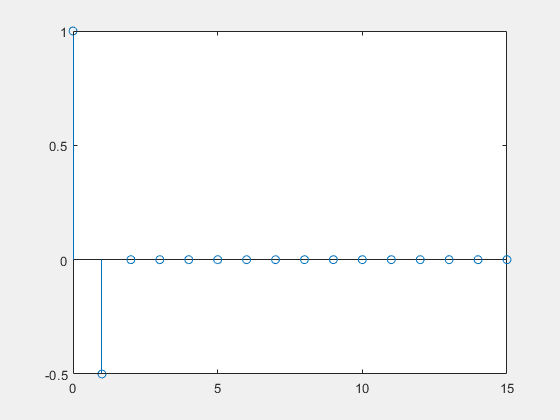
\includegraphics[width=0.45\textwidth]{../matlab/q26_2.png}
		\end{center}
		\caption{Response of inverse system \(\mathcal{S}_{3}\)}
		\label{fig:resp_s3}
	\end{small}
\end{figure}

\begin{figure}[htpb]
	\begin{small}
		\begin{center}
			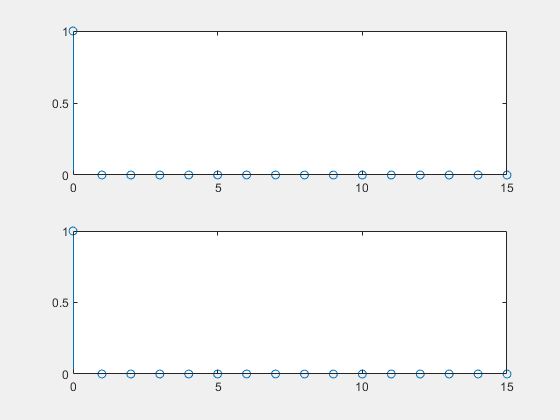
\includegraphics[width=0.45\textwidth]{../matlab/q26_3.png}
		\end{center}
		\caption{Impulse signal after \(\mathcal{S}_{2}\) and its inverse system}
		\label{fig:sig_inv_s2}
	\end{small}
\end{figure}

As Fig.\ref{fig:sig_inv_s2} shows, the impulse signal is recovered after passing the inverse system \(\mathcal{S}_{2}^{-1}\).

\section{Black Box Model Identification}

The justification of linearity and time-invariance of any given system can be easily utilized under MATLAB environment with its native support to function handles and vectorized signal operations. In another word, the theorems of linearity(\ref{linear_prop}) and time-invariance(\ref{ti_prop}) can be translated into MATLAB code with intuition.
\pagebreak
\begin{lstlisting}[language=matlab,style=matlab]
function ret=detNL(ufunc,tl1,tl2,tsL)
	%Boolean function justifies linearity of arbitary function @ufunc(x)
    ts1=rand([1,tsL]);
    ts2=rand([1,tsL]);
    test=ufunc(ts1*tl1+ts2*tl2)-ufunc(ts1)*tl1-ufunc(ts2)*tl2;
    ret=(max(abs(test))<=1e-5)*1;
end
\end{lstlisting}

\begin{lstlisting}[language=matlab,style=matlab]
function ret=detTV(ufunc,dt,paddle,tsL)
	%Boolean function justifies time-invariance of arbitary function @ufunc(x)
    ts1=[zeros(1,paddle),rand([1,tsL]),zeros(1,paddle)];
    ts2=circshift(ts1,dt);
    out1=ufunc(ts1);
    out2=ufunc(ts2);
    test=out2-circshift(out1,dt);
    ret=(max(abs(test))<=1e-5)*1;
end
\end{lstlisting}

The output of the two determining functions above indicates whether the unknown function \lstinline{@ufunc(x)}, where means the black-box function \lstinline{bboxN(x)}, satisfies linearity and time-invariance or not. A for-loop is adopted to apply the two determining functions to a list containing the handle of unknown functions that are demanded for determining:
\begin{lstlisting}[language=matlab,style=matlab]
	func_unkn={@bbox1,@bbox2,@bbox3};
	isnl=[];
	istv=[];
	%Global Variables
	for f=func_unkn
		a=detNL(f{1},randi(12),randi(12),120);
		b=detTV(f{1},randi(20),40,120);
		isnl=[isnl,a];
		istv=[istv,b];
	end
\end{lstlisting}

For the linearity, the justification output is
\begin{lstlisting}
isnl =
	1     1     0
\end{lstlisting}
indicating the non-linear function is \lstinline{bbox3(x)}. For the time-invariance, the output is
\begin{lstlisting}
istv =
	0     1     1
\end{lstlisting}
indicating the time-variant function is \lstinline{bbox1(x)}.

\section{Stock Market Example}
\paragraph{Filter 2.4}

The \lstinline{filter()} function in MATLAB automatically sets the initial conditions to zero if not providing further information of initial conditions by passing argument to this function. Therefore, applying the filter(2.4), which is illustrated in Fig.\ref{fig:7}, to the stock market data.
\begin{lstlisting}[language=matlab,style=matlab]
	f24 = [[0.2, 0]; [1, -0.8]];
	y1 = filter(f24(1, :), f24(2, :), rate);
\end{lstlisting}
Plot the output of the filter below:

\begin{figure}[htpb]
	\centering
	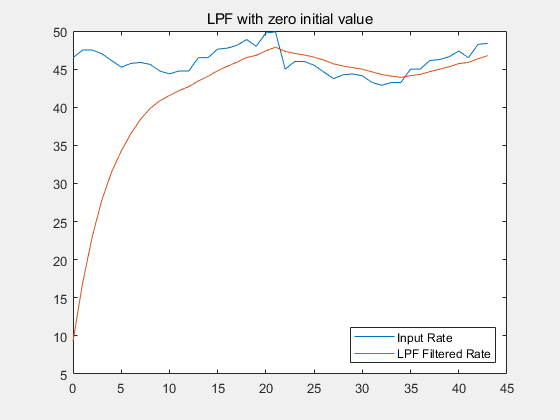
\includegraphics[width=0.35\textwidth]{../matlab/q28_1.png}
	\caption{1st-order LPF filtering result with \(y[-1]=0\)}
	\label{fig:q281}
\end{figure}

It's quite clear in the figure that the zero-initial output of the filter deviates dramatically at the initial, even though the output tracks up to the input smoothly along with the growth of time vector. This deviance shows more clear on the residue/smoothness plot Fig.\ref{fig:q283_rsp}.

\paragraph{Filter 2.5}

With the moving-average(MA) filtering there is no requirement of the initial conditions given. The filter output tracks up to the input quickly from zero and keeps a accurate tracking, for the MA filter is a FIR and it produces sharper response to its input. The MATLAB code is identical to the 1st-order IIR LPF above but the filter coefficients:
\begin{lstlisting}[language=matlab,style=matlab]
	f25 = [[1, 0, 0, -1] * 1/3; [1, -1, 0, 0]];
	y2 = filter(f25(1, :), f25(2, :), rate);
\end{lstlisting}
Plot the output of the filter below:

\begin{figure}[htpb]
	\centering
	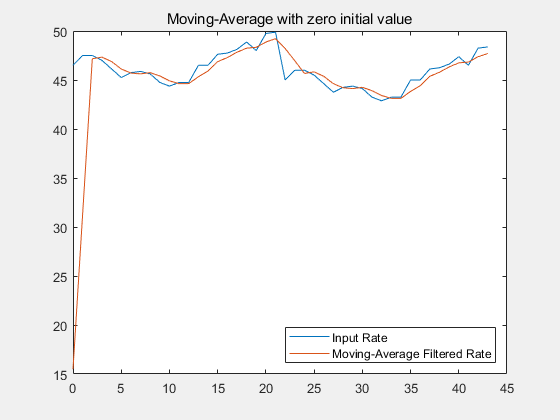
\includegraphics[width=0.45\textwidth]{../matlab/q28_2.png}
	\caption{3 Point Moving-Average filtering result}
	\label{fig:q282}
\end{figure}

The MA filter is sharper in tracking, but the smoothness of its output is worse than the result of 1st-order IIR filtering. This defect exposes more on the residue/smoothness plot Fig.\ref{fig:q283_rsp}.

\paragraph{Performance Comparation}
Use two criteria, the residue and 1st-order difference, to evaluate the accuracy and output smoothness of the two filters.
\begin{figure}[htpb]
	\centering
	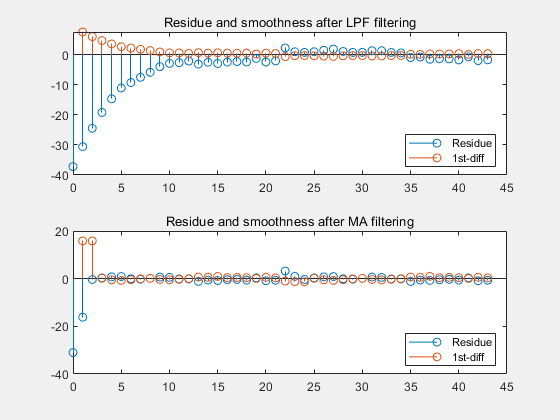
\includegraphics[width=0.45\textwidth]{../matlab/q28_3.png}
	\caption{Residue/Smoothness Plot}
	\label{fig:q283_rsp}
\end{figure}

The residue is difference between filter output and filter input, smaller residue indicates faster tracking and better performance, while smaller 1st-order difference means smoother output. It's obvious on the plot that the filter (2.4) boasts its better smoothness than filter (2.5), however the bad tracking speed of filter (2.4) make this filter much less applicant.

\paragraph{Initialing Filter (2.4)}

Initialize the filter (2.4) is equivalent to obtaining the zero-input response of the filter at \(0^{+}\). This is a essential problem in signal processing and system analyzing and can be solved by integration crossing \(t=0\):
\begin{equation}
	y(0^{+})=y(0^{-})+\mathcal{S}(x_{t<0})
\end{equation}

In discrete systems, this response can be simply calculated by solving the difference of the system with provided inputs and outputs before \(t=0\):
\begin{equation}
	\sum_{-\infty}^{-1}\alpha_{k}y[k]+\alpha_{0}y[0^{+}]=\sum_{-\infty}^{0}\beta_{k}x[k]\Rightarrow y[0_{+}]=\mathcal{S}(x_{t<0})+\sum_{-\infty}^{-1}\alpha_{k}y[k]
\end{equation}

There is an existing function \lstinline{filtic()} in MATLAB to perform this calculation. By intuition, the initial value at \(t=0\) can be selected as the initial condition at \(t=-1\) in best preservation of continuity. Substitute the evaluated IC(Initial Condition) into the filter and then obtain the output with better IC:
\begin{lstlisting}[language=matlab,style=matlab]
	f24 = [[0.2, 0]; [1, -0.8]];
	zi1 = filtic(f24(1, :), f24(2, :), rate(1));
	y1zi = filter(f24(1, :), f24(2, :), rate, zi1);
\end{lstlisting}

The poor tracking at the beginning of output is greatly improved, which is clearly shown on the input-output plot and the residue/difference plot Fig.\ref{fig:q284}:
\begin{figure}[htpb]
	\centering
	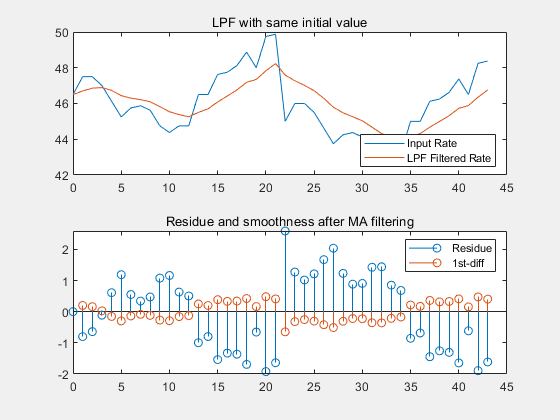
\includegraphics[width=0.45\textwidth]{../matlab/q28_4.png}
	\caption{MA filtering result with better IC}
	\label{fig:q284}
\end{figure}
This filter enjoys good tracking accuracy similar to filter (2.5), while preserving its better smoothness.

\end{document}